% % chapter 1 points:
% % - institutions matter, people aren't just touring
% % - everything has agloomed onto the religious level, which actually is eating away at clerical authority 
% %     - things that look like acts of faith don't automatically imply the growth of clerical power
    
% % chapter 2 points:
% % - bureaucratic representation is mixed in with tribal representation
% % - neat history of karbala
% % - religious rituals are fraught for clerics 
% % - what's really interesting is the repetition and oral history with opens traditions to changing, eating away at the clerical class

% % overall point:
% % - pious residents of a shrine city are paradoxically placed in terms of shaping religion
% %     - iraq's development has provided karbalaei natives with a powerful crux for shaping religion
% %     - religious rituals are fraught for clerics 
% %     - more religious != more clerical, especially for pious residents
% %     - oral traditions are ontologically open


% % Today the shrine institutions are poised to take over more parts of society from the receding state. 


% The Daura refinery in southern Baghdad was one of the few refineries to remain in operation during the entire Iraq-Iran war. Originally built in 1953 in what was then the outskirts of Baghdad, the refinery has come to be encircled by residential areas in prime real estate. While the founding intention was to have an oil refinery that would have easy access to the Tigris river for oil products, the upshot of its location is that the Daura refinery has come to shape Baghdad life, causing chemical runoff into the Tigris. 

% However, what is often overlooked is that the Daura refinery has acted in other roles, beyond the simple understanding of it as an actor of pollution and petrochemicals. The constant maintenance of the Daura refinery and the floating of balloons during the Iran-Iraq war to prevent Iranian bombings made it such that the refinery became a source of refuge. During the American invasion, the refinery became a fortress, with the manager of the refinery identifying it as a key part of Iraqi life in the capital. The Daura refinery has continued to become a source of expertise and experimentation, its privileged position as a jewel within Iraq's petrochemical crown has created repeated additions. 

% The Daura refinery shares many similarities with the bureaucracies of Karbala. Despite spending years under siege, the bureaucratic institutions has roared back to life, gobbling up the aspects of civil society that the government has left behind. In the vacuum left by a weak and dysfunctional post-2003 state, the shrine institutions of Karbala provided a continual source of expertise in management of local power struggles, being one of the few organizations with institutional knowledge that survived 2003. In the wake of ISIS and collapse of the Iraqi army, the rise of the Hashd al-Shaabi, legitimized by Ayatollah Sistani's fatwa and funded in part by Iran has created a parallel army, just as the shrine institutions have created parallel bureaucracies. 

% However, the key difference is that while the state army and bureaucracy is supposed to be non-sectarian, the Hashd and Shrine institutions are avowedly Shi'a. Using the guise of religion both groups have expanded their control over physical territory, which simultaneous dilutes the meaning of religion. As more things become affiliated with religion, authority becomes diluted as well, with more ways to practice religion outside of the auspices of the clerical class. 

% The strong history of organization outside the traditional religious authorities within tribal affairs and \emph{muwālkib} have provided a frame that allows for the laity to assert itself, as well providing a door for political influence, such as Iran's influence. This has resulted in Shi'ism in South Iraq becoming a tapestry as multiple groups seek to assert what it means to be Shi'a. The existence of Shi'a rituals means that each group, whether it is the laity, the clerical class, the militias, or the Karbala institutions, has a chance to define and refine its own definitions of religiosity. 

% % This change in clerical 

% % Not only is Karbala shrines a story of Karbala corruption, these institutions themselves are transformed by the aspects around it. This is not a story unique to Iraq, but the merging of major state controlled industries combined with near automatomous bureaucracies have resulted in an expansion of what is deemed religious. Under the guise of religion, groups such as the Hashd al-Shaabi and the Imam Hussein Shrine have expanded their domains at the cost of the state, which has resigned itself to being unable to manage alone. 

During Arbaeen, while walking from Najaf to Karbala, I passed by a \emph{mūkeb} which featured cardboard cutouts of both Qassem Soleimani and Abu Mahdi Muhandis, two men who were killed by the United States in early 2021. Qassem Soleimani led the Quds Brigades, an Iranian military branch, while Abu Mahdi Muhandis was the leader of the Hashd al-Shaabi and a key partner for Soleimani. Next to the cutouts, pictures of martyrs adorned the walls next to mock graves. Multiple banners were placed above the pictures of martyrs, with a large photo of Ayatollah Sistani is juxtaposed with another large photo of Abu Mahdi Muhandis. A loudspeaker was blaring a \emph{latmiya}. Close by, volunteer of this \emph{mūkeb} provided food and water for pilgrims.

A few pilgrims would stop and take photos with the cutouts, holding hands with both cutout men. Others would stop and contemplate wall of marytr photos, as women wailed leaned over the mock graves and wailed.

While waiting in line for a falafel at this \emph{mūkeb}, I asked a few people for their thoughts. An Iranian man who spoke Arabic remarked to me that "the Iraqis love him [Qassem Solemani] more than we do!" An Iraqi man noted that he quite liked the cut-outs, and found it amusing that people would come and take photos with the cutouts. When taking my falafel, I asked the volunteer making food whether he was affiliated with the Hashd, and if there was a \emph{radūd} present. He responded that he was merely a volunteer from a nearby village and wanted to help pilgrims, and that the \emph{radūd} was sleeping. 

\begin{figure}[h]
\caption{A mowkeb dedicated to the martyrs of the Hashd. Image taken by the author, August 2022.}
\centering
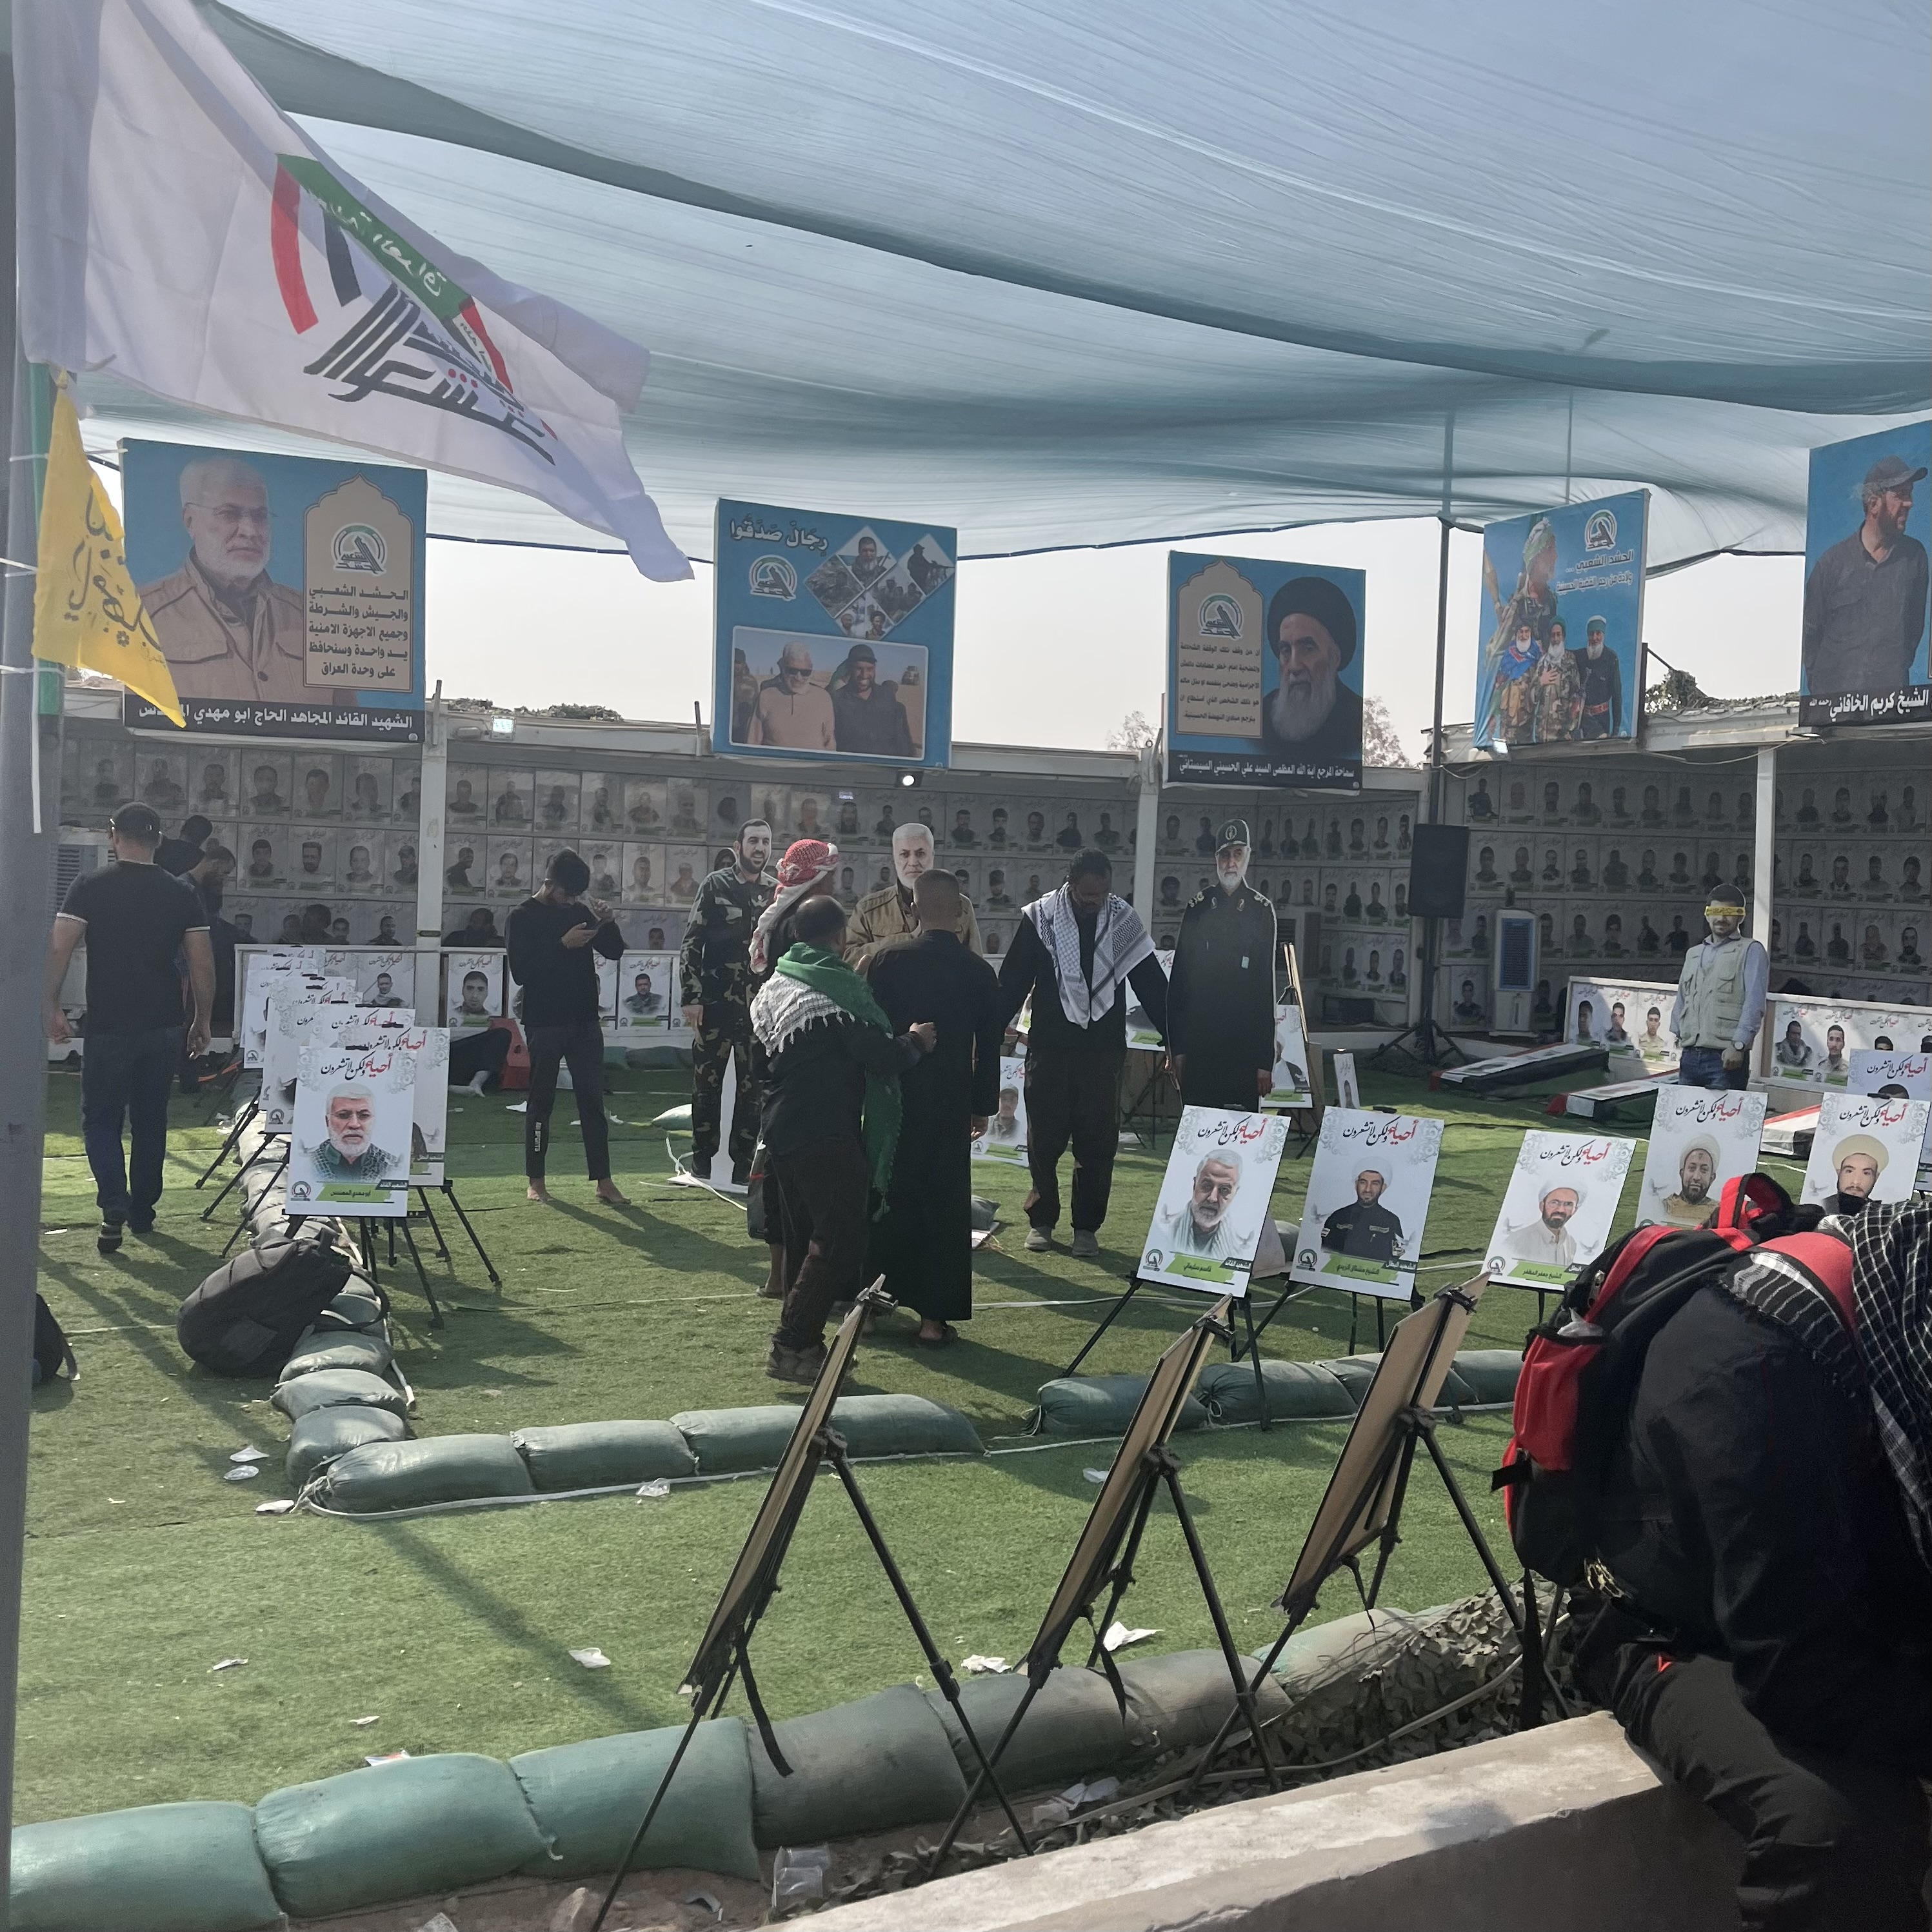
\includegraphics[width=.75\textwidth]{images/qassem-mowkeb.jpeg}
\label{fig:qassem-mowkeb}
\end{figure}

Such encounters are examples of the themes I have talked about in this thesis. Pilgrim attention creates a public that is overflowing with motifs, from the pictures of Sistani and Muhandis situated on the same eyeline, to the physicality of mock graves and cutouts, to the auditory experience of the \emph{latmiya} from the speakers, to the food provided by the \emph{mūkeb}. Pilgrims are drawn in a multitude of ways, enticed to take photos, eat food, or participate in a \emph{latm}. 

In Chapter \ref{chapter-1} I talked about how the tension between \emph{rawadīd} and the Hashd al-Shaabi militias reveal competing sources of authority and power within the Shiite community. As both groups lay claim to different forms of religious legitimacy and political influence, they challenge the monopoly of clerical authority over religious and moral guidance. Public sphere theory can shed light on how these alternative publics challenge and redefine the boundaries of religious authority and contribute to the changing nature of clerical authority. 

In Chapter \ref{chapter-2}, I discussed how the institution of \emph{mūkeb} demonstrates that clerical authority has always been historically negotiated and contingent upon local contexts. The \emph{muwālkib} allows for the formation of publics and communities outside the direct control of religious institutions, thereby enabling alternative forms of religious expression, social organization, and political mobilization. Saba Mahmood's work on agency and subjectivation provides a useful framework for understanding how these competing groups negotiate their roles and assert their agency within the religious landscape.

A possible point of departure for future research is the register of tragedy. All Shi'a rituals are infused with the register of martyrdom, which this thesis has largely ignored. Additional research could be conducted on if and how the register of tragedy and sacrifice allow for a specific construction of self, and whether the public acknowledgement of martyrdom, which is everywhere in Iraq, help to create new identities. 

It is essential to recognize that clerical authority in southern Iraq is not static or monolithic, nor is it solely determined by the religious and political dynamics in Najaf. By engaging with both public sphere theory and Saba Mahmood's work on agency and subjectivation, and by expanding our analysis to consider a broader range of actors and institutions, we can gain a deeper understanding of the complex dynamics that shape religious authority, political power, and the shifting landscape of religious and communal life in southern Iraq.